\documentclass[11pt]{article}
\usepackage{amsmath}
\usepackage[margin=0.68in]{geometry}
\usepackage{booktabs}
\usepackage{enumitem}
\usepackage{fancyhdr}
\usepackage{graphicx}
\usepackage[table]{xcolor}
\usepackage[hidelinks]{hyperref}
\usepackage{listings}
\usepackage{microtype}
\usepackage{tabularx}
\usepackage{titlesec}
\graphicspath{{docs/design/drafts/lesson-037/assets/}{assets/}}
\definecolor{Ink}{gray}{0}
\definecolor{CodeGray}{gray}{0.96}
\hypersetup{hidelinks,pdftitle={ADK Lesson 037: Contact Dynamics},
 pdfauthor={Kevin Shanahan},
 pdfsubject={Host-independent contact qualification, refractory policy, and supplied-trace evidence},
 pdflang={en-US}}
\pagestyle{fancy}\fancyhf{}
\lhead{\textsc{ADK Lesson 037}}\rhead{Contact Dynamics}
\cfoot{\thepage}\setlength{\headheight}{14pt}
\setlength{\parindent}{0pt}\setlength{\parskip}{5pt}
\setlist{nosep,leftmargin=1.45em}
\titleformat{\section}{\Large\bfseries\color{Ink}}{\thesection}{0.5em}{}
\lstdefinestyle{adkcpp}{language=C++,backgroundcolor=\color{CodeGray},
 basicstyle=\ttfamily\small,keywordstyle=\color{Ink}\bfseries,
 commentstyle=\color{Ink},columns=fullflexible,keepspaces=true,
 showstringspaces=false,frame=single,rulecolor=\color{Ink},
 breaklines=true,tabsize=4}
\newcommand{\lessonbox}[1]{%
 \begin{center}\fcolorbox{Ink}{white}{\parbox{0.92\linewidth}{#1}}\end{center}}

\begin{document}
\lessonbox{\textbf{NONCANONICAL DESIGN DRAFT --- NOT PUBLISHED.} This file is
review material under \texttt{docs/design/drafts}. It is not a released
lesson, site page, download, Mega example, schematic, or support claim.}

\begin{center}
 {\Huge\bfseries Contact Dynamics}\\[4pt]
 {\Large Turn a supplied level trace into one qualified contact}\\[8pt]
 \textit{Observe every sample, qualify time, suppress repeats}
\end{center}
\begin{tabularx}{\linewidth}{@{}>{\bfseries}l X >{\bfseries}l X@{}}
Lesson & 037 --- component & Time & 90--150 minutes\\
Prerequisites & Lessons 006 and 007 & Fixture & timestamped host trace\\
Evidence & snapshots and replay comparison & Status & host-independent draft\\
Energy class & E0 pure behavior; no powered specimen\\
\end{tabularx}

\lessonbox{\textbf{Scope gate.} This edition uses supplied timestamped
\texttt{Level} values only. It does not authorize a retail module, capsule,
contact, piezo element, Mega pin assignment, LED panel, or powered circuit.
Exact-specimen identification, primary electrical evidence, an authoritative
schematic, current accounting, a canonical Mega example, and bench acceptance
remain open.}

\section{Mission and vocabulary}
Mechanical contacts can chatter: one action may produce several rapid level
changes. This lesson separates what was sampled from what policy accepts:
\[
\text{raw level}\rightarrow\text{qualified contact}
\rightarrow\text{attack event}\rightarrow\text{release event}.
\]
\texttt{ContactDynamics} consumes copied observations. It does not measure
force, acceleration, impact energy, orientation, damage, or safety. Fixture
names such as \texttt{shortPulse}, \texttt{chatterTrain}, and
\texttt{heldContact} describe waveform shape, not a retail sensor.

\section{Read the trace in dependent stages}
\begin{center}
% ADK visual: pencil
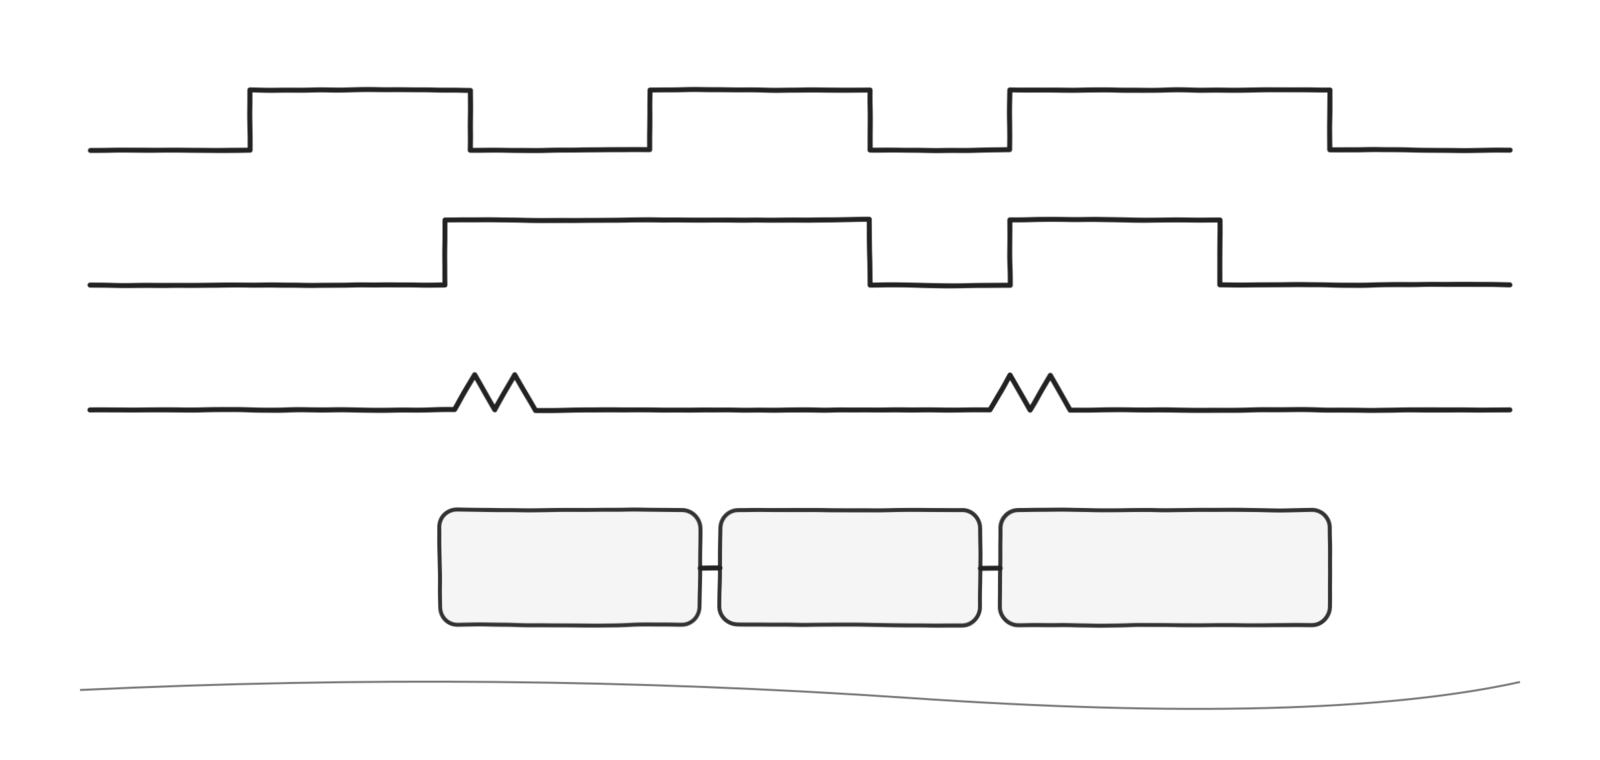
\includegraphics[width=0.98\linewidth]{037-contact-stages-pencil.png}

\small\textit{Alternative text: a pencil timeline follows copied inactive and
active levels through a qualification interval, one accepted attack,
refractory suppression, a qualified release, and an explicit held-active
warning; raw evidence remains visible beneath each interpretation.}
\end{center}

An attack candidate must remain continuously active for \texttt{qualify}.
Acceptance is timestamped by the update that completes that interval. A
qualified release likewise needs continuous inactivity for \texttt{release}.
One held contact cannot manufacture repeated attacks.

Refractory time starts at an accepted attack. An attack completing before its
exact boundary is suppressed; completion exactly at the boundary is accepted.
Suppression remains evidence through its disposition and saturating counter.
The stuck-active clock starts at accepted attack, not at the first noisy edge.

\section{Contract and snapshot}
\texttt{ContactDynamicsConfig} selects active level and four nonzero,
half-range-safe durations: qualification, release, refractory, and
stuck-active. Construction is inert. \texttt{initialize()} validates policy,
\texttt{update(sample)} processes one copied observation, \texttt{snapshot()}
does not consume evidence, and \texttt{reset()} clears time history and
counters.

\begin{tabularx}{\linewidth}{@{}l X@{}}
\toprule
Snapshot evidence & Interpretation\\
\midrule
\texttt{rawLevel}, \texttt{rawActive} & the supplied sample, before policy\\
\texttt{qualifiedActive} & continuously active long enough to qualify\\
\texttt{attackEvent}, \texttt{releaseEvent} & event produced by this update only\\
\texttt{qualifiedPulseWidth} & accepted attack to qualified release\\
\texttt{refractoryRemaining} & bounded suppression interval still open\\
\texttt{acceptedCount}, \texttt{suppressedCount} & saturating history\\
\texttt{disposition} & none, accepted, or suppressed on this update\\
\texttt{quality}, \texttt{status} & validity or explicit source/timing fault\\
\bottomrule
\end{tabularx}

Before the first successful sample, quality is
\texttt{Unqualified}. A non-Ok source sample reports
\texttt{SourceFault}, creates no event, and requires reset before
qualification resumes. \texttt{update()} can also receive a malformed enum
value such as
\texttt{static\_cast<Level>(7)} from an unsafe adapter boundary. It reports
\texttt{InvalidArgument} with \texttt{SourceFault}, creates no event, and
likewise stays faulted until reset. Continuous accepted activity reaching
\texttt{stuckActive} reports \texttt{StuckActive}; a later qualified release
returns current quality to \texttt{Valid}. Counts preserve the history.

\section{Time is supplied evidence}
Time enters only in \texttt{ContactSample}. Natural 32-bit rollover is valid.
An apparent jump at or beyond the unsigned half-range is a timing fault and
must not partially mutate state. An identical same-time sample is idempotent;
changed evidence at the same time is invalid.

One-update fields---attack, release, and disposition---clear on the next later
update. Stable snapshots let a caller inspect the same result more than once
without consuming it. This polling interface cannot reveal level changes that
occur entirely between supplied samples. It also cannot reconstruct the exact
edge time: event time is the update that proves the duration.

\section{Run four supplied-trace experiments}
\begin{center}
% ADK visual: pencil
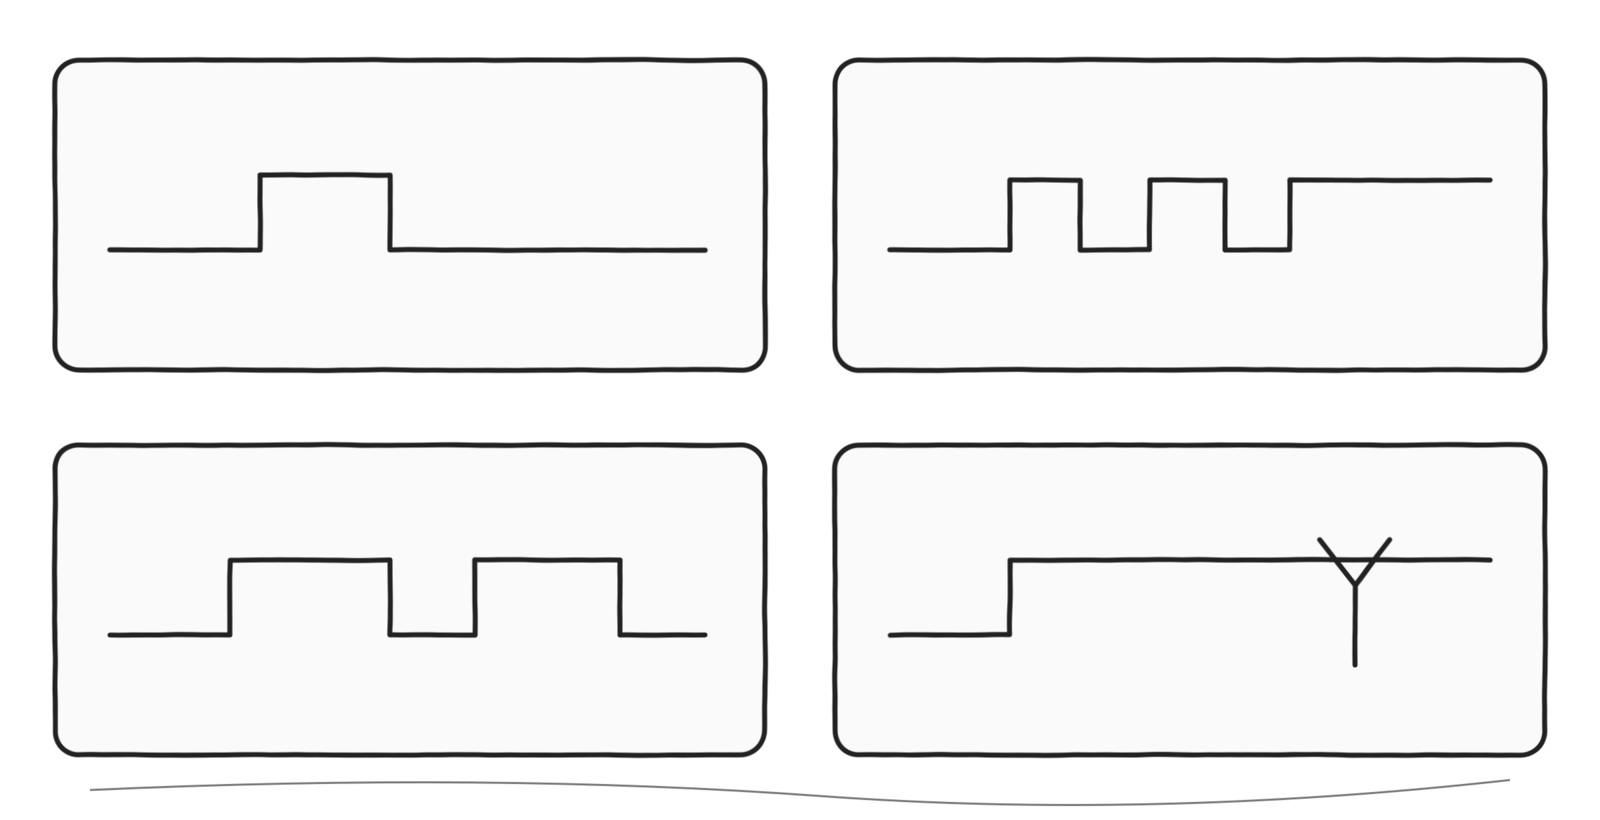
\includegraphics[width=0.98\linewidth]{037-trace-lab-pencil.png}

\small\textit{Alternative text: four pencil laboratory cards show a short
pulse rejected before qualification, a chatter train settling into one
attack, two attacks with the second suppressed during refractory, and a held
contact crossing the stuck-active boundary before release.}
\end{center}

For every experiment, write the predicted snapshot rows before replay. Observe
the complete snapshot after each timestamp, then interpret only the policy
supported by those rows.

\begin{enumerate}
 \item \textbf{Short pulse.} Supply active evidence for less than
       \texttt{qualify}. Predict no attack and no count change. Interpret this
       as insufficient duration, not proof that no physical action occurred.
 \item \textbf{Chatter train.} Alternate levels, then hold active through the
       boundary. Predict candidate restarts on every break and exactly one
       accepted attack. Interpret the accepted timestamp as qualification
       time, not the first raw edge.
 \item \textbf{Refractory pair.} Qualify, release, then qualify again before
       refractory expiry. Predict one accepted and one suppressed count.
       Repeat with completion exactly at expiry and predict acceptance.
 \item \textbf{Held contact.} Keep qualified activity through
       \texttt{stuckActive}, then supply a qualified release. Predict no
       repeated attack, a temporary stuck quality, one pulse width at release,
       and recovery to current Valid quality.
\end{enumerate}

\section{Replay one trace exactly}
Use an active-low configuration:
\[
\texttt{qualify}=30\text{ ms},\quad
\texttt{release}=20\text{ ms},\quad
\texttt{refractory}=80\text{ ms},\quad
\texttt{stuckActive}=120\text{ ms}.
\]
Initialize once, then submit the rows in order. Every status is
\texttt{Ok}. A dash means neither one-update event is expected.

\begin{tabularx}{\linewidth}{@{}r l X X@{}}
\toprule
Time (ms) & Level & Predict & Key observation\\
\midrule
0   & High & idle & Valid, counts 0/0\\
10  & Low  & candidate starts & raw active; not qualified\\
20  & High & chatter breaks candidate & no attack\\
30  & Low  & candidate restarts & raw active; not qualified\\
60  & Low  & accepted attack & attack, Accepted, counts 1/0\\
70  & High & release candidate & still qualified\\
90  & High & qualified release & release, pulse width 30 ms\\
100 & Low  & second candidate starts & refractory still open\\
130 & Low  & suppressed attack & attack, Suppressed, counts 1/1\\
\bottomrule
\end{tabularx}

For the held-contact experiment, call \texttt{reset()}, then submit
\texttt{(0,High)}, \texttt{(10,Low)}, \texttt{(40,Low)},
\texttt{(160,Low)}, \texttt{(170,High)}, and \texttt{(190,High)}, all Ok.
Predict acceptance at 40 ms, \texttt{StuckActive} at 160 ms, and a qualified
release with 150 ms pulse width at 190 ms.

\begin{lstlisting}[style=adkcpp]
ContactDynamicsConfig config (
    Level::Low, Duration (30), Duration (20),
    Duration (80), Duration (120));
ContactDynamics dynamics (config);
require (dynamics.initialize ().ok ());

for (const ContactSample& sample : trace)
{
    Status status = dynamics.update (sample);
    saveFields (status, dynamics.snapshot ());
}
requireCompleteFieldEquality (
    savedFirstRun, replayFromReset (config, trace));
\end{lstlisting}

The harness must save the complete status and snapshot after every row, not
only event rows. Construct a fresh component or call \texttt{reset()} before
each independent trace. For the malformed-level case, submit:
\begin{lstlisting}[style=adkcpp]
ContactSample {TimePoint (200), static_cast<Level> (7), StatusCode::Ok}
\end{lstlisting}
Verify \texttt{InvalidArgument}, \texttt{SourceFault}, no event, and continued
fault on a later well-formed sample until reset.

\section{Predict, observe, interpret worksheet}
\begin{tabularx}{\linewidth}{@{}p{0.20\linewidth} X X@{}}
\toprule
Stage & Record before replay & Compare after each update\\
\midrule
Predict & event timestamp, disposition, counts, quality & no fixture result yet\\
Observe & do not revise the prediction & raw, qualified, event, time, status\\
Interpret & contract claim the evidence supports & mismatch and next trace edit\\
\bottomrule
\end{tabularx}

A mismatch is useful only when retained exactly. Save the configuration,
timestamps, levels, statuses, and every named snapshot field. Replay the same
typed inputs and compare every field, including \texttt{Status::error()}.
Never compare raw C++ object bytes: padding has no canonical meaning.

\section{Diagnosis}
\begin{tabularx}{\linewidth}{@{}X X@{}}
\toprule
Observation & Inspect next\\
\midrule
attack never appears & active level, continuous duration, sample spacing\\
several attacks from one hold & candidate reset and held-contact policy\\
second attack accepted too early & refractory start and exact-edge comparison\\
release pulse width stays zero & continuous inactive release qualification\\
source fault followed by an event & reject the run; reset is required\\
rollover faults unexpectedly & use modular elapsed time and half-range rule\\
\bottomrule
\end{tabularx}

\section{Exercises and limits}
\begin{enumerate}
 \item Construct the smallest trace that accepts exactly at qualification.
 \item Change one same-time level and explain why replay must fault.
 \item Draw a valid qualification interval across natural rollover.
 \item Explain why a suppressed attack remains important evidence.
 \item Increase sample spacing and identify which short pulses become
       unobservable without claiming they never happened.
\end{enumerate}

\lessonbox{\textbf{Stop rule.} Keep this edition host-independent. Do not
connect or power an unknown contact, glass capsule, tilt switch, tap/shock
module, microphone board, or bare piezo. Do not infer polarity, pin order,
voltage range, pull-up rail, or safe current from a listing name.}

\section{What the result establishes}
A passing supplied-trace replay establishes deterministic qualification,
release, refractory, stuck-active, fault, rollover, and snapshot behavior for
the exact samples provided. It does not establish the identity or electrical
safety of a specimen, physical edge capture between polls, force or impact
measurement, a Mega circuit, or bench performance.

The sibling Markdown design draft provides searchable review prose. This
locally compiled PDF draft remains untagged, unpublished, and makes no PDF/UA
claim. A later exact-specimen gate must add
primary evidence, wiring and current review, an authoritative formal
schematic, a canonical Mega example, visible non-Serial evidence, measured
safe-state checks, and a recorded human bench result.
\end{document}
